\documentclass[../main/thesis_msc.tex]{subfiles}

\begin{document}

\chapter{Magnetic field study at Low frequency}

\section{Introduction}

For several decades, the magnetic fields seen the galaxies have mystified astronomers. One of the main motivations behind studying these fields is to understand their contribution in the evolution of galaxies. Several questions about the magnetic fields needed to be answered such as whether magnetic field is just a consequence of the motion of the charged particles, or whether it influences the evolution. As charged particles are present pretty much every where, including the cold atomic clouds, magnetic field can exist every where in the galaxy. One of the first measurements of the magnetic fields in the nearby galaxies was done for the Andromeda galaxy (M31) in 1958. Interstellar linear polarization in Milky Way was studied in terms of extinction of selective elongated dust grain particles (the Davis-Greenstein effect). These particles get aligned by the magnetic field and hence provide us with the understanding of the interstellar magnetic fields which were parallel to the Galactic plane \citep{2008ApJ...676L..25L}. To get a better understanding of the history of study of polarization in radio frequencies, one may refer to \citet{2013pss5.book..641B}. \\
\noindent One of the most important forces in the study of magnetic fields, is the Lorentz force\footnote{It is the force experienced by a charged particle in the presence of an electric (\textbf{\textit{E}}) and magnetic (\textbf{\textit{B}}) field and is written as: \textbf{\textit{F}} = q\textbf{\textit{E}} + q(\textbf{\textit{v}} + \textbf{\textit{B}}).}, through which they influence the Interstellar Medium (ISM). Thus, the magnetic fields are some of the main contributors to the dynamical activity in galaxies. Relativistic electrons, through synchrotron emission, help us study the perpendicular magnetic field component \textbf{\textit{B}}$_{\bot}$. The degree of polarization of this emission is around 75\%, though the actual measured quantity is much less. \\
%Stokes parameters described the the earlier chapters can help us obtain this component of the magnetic field. Let us consider the total polarized \\
%\begin{equation}
%I_{pol} = \sqrt{U^2 + Q^2 + V^2}
%\end{equation}

In the recent years, two methods have been proposed to study the parallel component of the magnetic field in astronomical objects:
\begin{itemize}
\item \textbf{Zeeman splitting:} Splitting of an atomic or molecular line in the presence of a magnetic field is called Zeeman splitting. Amplitude of the Zeeman splitting, $\bigtriangleup\nu \propto \textbf{\textbf{B}}$, with \textbf{\textbf{B}} being the magnetic field. Hence, by measuring the $\bigtriangleup\nu$ one can measure the magnetic field. However, since the value of $\bigtriangleup\nu$ is very small, we use the measurement from the Right Circular Polarization (RCP) and the Right Circular Polarization (RCP) to find the $\textit{\textbf{B}}_{||}$. This measures more of the cold neutral cloud regions. Using this method, for the first time, H I observations of Cas A gave its magnetic fields.
\item \textbf{Faraday rotation (FR) of linearly polarized light:} In the presence of a magnetic field (like in an ionized medium), the electromagnetic field has a right-hand (RH) mode, that is when the electric field is along the direction of motion of the gyrating electron and a left-hand (LH) mode that is when the electric field is in the opposite direction to the motion of the electron. The RH mode Electric field travels faster than the LH mode because of the interaction between the electric field and the electron. This in turn results in the rotation of the plane of polarization. The rotation angle $\psi$ of a polarized radio wave is given by the equation \ref{eq}, where $\lambda$ is the wavelength of the observation (in m) and RM is the rotation measure in rad m$^{-2}$. 

\begin{equation}
\textrm{RM} = \frac{\partial \psi}{\partial \lambda^2}
\label{eq}
\end{equation}

where the angle of polarization can also be written as:
\begin{equation}
\psi = \frac{1}{2} tan^{-1} \frac{U}{Q}
\end{equation}
\end{itemize}
In theory, one may obtain the RM by plotting the angle of polarization against the $\lambda^2$. However, this is not feasible in real life because of several reasons, such as the $n\pi $ ambiguity. This effect is seen because the polarization angle is known only know in multiples of $\pi$. Hence, with a few wavelength bands, this fitting would just be arbitrary (for example in \citet{1994MNRAS.268..497R}). Another major reason is depolarization, which is notably seen at lower frequencies. It was first observed in the paper \citet{2010iska.meetE..58W} for LOFAR. In this paper, it was seen that an unpolarized source was showing significant signal in the XY/YX correlations, and none in XX/YY. With the help of the RIME, this phenomenon can be mathematically explained. It can be shown that if a 1~Jy source undergoes a FR of $\pi / 2 [+2\pi $n$]$ on one of the stations and 0[+2$\pi$n] on the other station, all the original I flux will be detected as V. This phenomenon was termed as Differential FR. At the low frequencies in which LOFAR operates, ionospheric FR can be very high, making the observation of polarization significantly harder.\\
\noindent There are four major depolarizations seen other than wavelength dependent depolarization.
\begin{itemize}
\item \textbf{Bandwidth dependent depolarization}: This kind of depolarization occurs when the signal get depolarized within a frequency band. The polarized signal is reduced proportional to the sinc of the bandwidth (in terms of $\lambda^2$). This effect can be reduced by dividing the whole bandwidth into narrower channels. 
\item \textbf{Beam depolarization}: If the magnetic field is tangled on scales that are smaller than the resolution of the observation, some of the polarization is canceled out by itself inside the beam. This effect can be reduced by having better resolution.
\item \textbf{Faraday dispersion}: The polarized emission sometimes is depolarized through by Faraday rotation the line of sight (LOS). If this occurs within the emission region, it is called internal, and if it is outside, it is called external. 
\item \textbf{Galactic foreground}: If the galaxy is present at lower galactic latitudes, this polarization becomes very important. It is caused by the polarization by the Milky Way galaxy. It is an example of external Faraday dispersion.
\end{itemize}

\noindent In order to curb the effects of the limited sampling of $\lambda^2$, the technique of RM Synthesis is used as described in \citet{2005A&A...441.1217B}, which is the continuation in the work done in the paper \citet{1966MNRAS.133...67B}. This method is described in the next section.\\ 
\section{Faraday Rotation Measure synthesis technique}
\noindent Faraday depth ($\phi$) of a source can be written as in equation \ref{rm}. Here, $\textit{\textbf{B}}_{||}$ is the parallel component of the magnetic field (in $\mu$G), $n_e$ is the free electron density in cm$^{-3}$ and $dl$ is the path length in parsec\footnote{\textbf{Note:} One must remember that Rotation Measure is the same as Faraday Depth if and only if the Faraday rotating medium is present in front of the background source. If an emitting plasma exists in the source, then the equation can only be written in terms of $\phi$. Thus, Faraday Depth is the general case and the RM is used for a specific case only.}.
\begin{equation}
\phi(\textbf{r}) = 0.81 \int_{\textrm{here}}^{\textrm{there}} n_e \textit{\textbf{B}}_{||} dl \textrm{  (rad m}^{-2})
\label{rm}
\end{equation}

\noindent The polarization vector can be written in terms of the polarization angle as:
\begin{equation}
P(\lambda^2) = \int^{+\infty}_{-\infty} pIe^{2i[\psi_0 + \phi \lambda^2]}d\phi
\end{equation}
Faraday dispersion function describes the intrinsic polarized flux, and can be written in terms of Faraday depth. Thus, we can wrote Faraay depth as $F(\phi)= pIe^{2i\psi_0}$. Thus, the relation is in the form of a Fourier transform, and can be inverted to give:
\begin{equation}
F(\phi) =  \int^{+\infty}_{-\infty} P(\lambda^2) e^{-2i\phi \lambda^2} d\lambda^2
\end{equation}
However, we do not observe for wavelengths in which $\lambda^2 < \infty$ and \textit{all} the values in which $\lambda^2 > 0$. Hence this technique was formulated. It also avoids bandwidth depolarization by averaging the complex polarization. The reconstructed Faraday dispersion function is thus written in the form described in equation \ref{rmsf}. $R(\phi)$ is the Rotation Measure Synthesis Function (RMSF). 
\begin{alignat}{2}
  &&F'(\phi)&=F(\phi) * R(\phi)\\
  &&&= K\sum\limits^{N}_{i=1} w_i P_i e^{-2i\phi(\lambda_i^2 - \lambda_0^2)}
\label{rmsf}
\end{alignat}
Here, $*$ denotes convolution. $w_i$ is the weight of the $i^{th}$ data point. The RMSF represents the response of the instrument because of the discrete separation of the bandwidth into separate channels. It is: 

\begin{alignat}{2}
  &&R(\phi)&= K\sum\limits^{N}_{i=1} w_i e^{-2i\phi(\lambda_i^2 - \lambda_0^2)}\\
  &&K& = \frac{1}{\sum\limits^{N}_{i=1} w_i}
\end{alignat}

\noindent Once RM Synthesis has been performed, a deconvolution procedure called RM Clean is performed to get rid of the side lobes generated by the RMSF \citep{2009A&A...503..409H}. These side-lobes provide difficulties in obtaining the Faraday Depth at which the source is present. This deconvolution is somewhat similar to the one performed during the imaging synthesis procedure. The flow chart in Figure \ref{rmsynth} describes the different steps in performing RM Synthesis. \\
\begin{figure}[h]
\centering
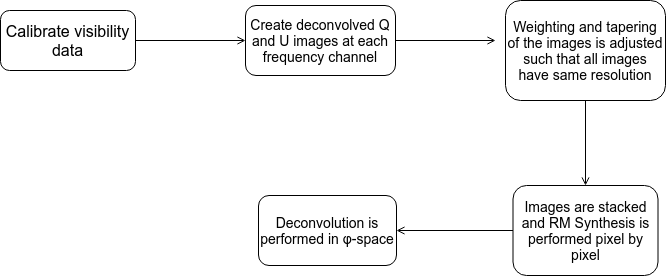
\includegraphics[scale = 0.5]{rmsynth.png}
\caption{Flow chat depicting the procedure of RM Synthesis to understand polarization in astronomical objects, using the visibilities obtained from a radio receiver}
\label{rmsynth}
\end{figure}

\noindent \textbf{Caveats:} Some of the limitations of the RM Synthesis is described below:
\begin{itemize}
\item The deconvolution process may amplify the artifacts, thus decreasing the image quality.
\item The higher and lower frequency images need to be of the same resolution, resulting in the loss of resolution of the higher frequency images due to the tapering and the convolution processes involved. 
\item Wide continuous frequency range is required to see the magnetic field structures in spiral galaxies.
\end{itemize}
There are other methods to obtain Rotation Measures- Faraday Synthesis \citep{2012AA...540A..80B}, \citep{2009A&A...503..409H} which is followed by clean, wavelets \citep{2010MNRAS.401L..24F}, compressive sampling \citep{2011A&A...531A.126L}, and QU-fitting \citep{2011AJ....141..191F}. In the first three methods, the Faraday spectra is decomposed into some basis function. In the last method- QU fitting, models of synchrotron-emitting and Faraday rotating medium to the observed $P(\lambda)$ are assumed. In the paper \citet{2015AJ....149...60S}, the various methods were compared with each other to figure out which algorithm works the best to reconstruct the Faraday Spectra. The test was run on 1.1 to 1.4~GHz data with a SnR of 32 to 15. It was found that errors in the Faraday Depth weighted by polarized intensity were sometimes almost a magnitude higher for the first three methods (Faraday Synthesis, wavelets and compressive sampling) than the errors from the QU fitting algorithm. Most of these methods worked well for Faraday thin sources\footnote{A Faraday thin source is one in which $\lambda^2 \vartriangle \phi << 1$, with $\vartriangle \phi$ denoting the extent of the source in terms of Faraday Depth ($\phi$). These sources are well approximated by a Dirac-$\delta$ function of $\phi$.}, while for Faraday thick structures\footnote{A Faraday thick source is one in which $\lambda^2 \vartriangle \phi >> 1$, and it is extended in faraday depth. Such a source is considerably depolarized in $\lambda^2$.} all the methods fail. QU-fitting seems to have performed much better than the other methods.  

\section{Faraday tomography of the galaxies}
The study of linear polarization helps us to understand the magnetic fields within the source through synchrotron polarization and Faraday rotation, and also through the LOS to the source with the help of Faraday rotation. Ideally, LOFAR would be a very good instrument to measure the polarization because it has the potential to measure to measure the Faraday depths to an accuracy of 0.1 rad/m$^2$. It can also indicate the presence of two polarized sources which are separated only by a few rad/m$^2$. It could, in principle, measure weak magnetic fields and detect low electron densities that are not observable at higher frequencies.\\


\paragraph{Magnetic fields in IC\,342:} Studying magnetic field for IC\,342 at such a low frequency would be very interesting, because it has a high star formation rate at the center, unlike most of the other spiral galaxies, in which the star formation mostly takes place in the spiral arms. The high SFR at the center could be attributed to the inflow of gas from the outer parts of the galaxy in a steady form. In the Figure 27 in the paper \citet{2015A&A...578A..93B}, one can clearly see the ``magnetic arms" of the galaxy pointing towards the center. The magnetic fields in the galaxy have been studied thoroughly at lower wavelengths such as 20.1~cm using VLA, in which it was found that depolarization effects dominate in the northern part of the galaxy, given the galaxy's receding rotation. This is attributed to the galaxy's helical fields that are present from the disk to the halo of the galaxy, as predicted by the mean-field dynamo models (see \citet{2015A&A...578A..93B} for more information on this). It has also been studied at a wavelength of 6.3~cm and 11.1~cm using the Effelsberg telescope, where it was first found that the galaxy has an axisymmetric spiral field \citep{grave}. The degree of polarization at the two wavelengths were about 13\% and 10\% respectively.

\paragraph{Magnetic fields in NGC\,628:} To study the magnetic fields of the disks of spiral galaxies, NGC\,628 is one of the best as it is an almost-face on galaxy with a low inclination of around 7~deg. It is also an isolated galaxy (like IC\,342), which would facilitate mean field dynamo to operate without any major disturbance. In the paper \citet{2017A&A...600A...6M}, NGC\,628 was found to have an ordered magntic field along the northern arm (in the regions \textbf{A} and \textbf{B} of the figure \ref{hlaph_ng}), with a high degree of polarization, possibly being caused by an asymmetric HI hole. A three dimensional field deviation called Parker loop which results in periodic small scale variations of the field orientation and position angle is seen in the northern arm (caused by Parker instability\footnote{A net force on the plasma that leads to its acceleration caused by magnetic buoyancy is called \textbf{Parker instability}.}). High level of polarization is seen in the inter arm regions, as observed in IC\,342 (see Figure 28 of the paper to see the magnetic field lines). 

\subsection{RM Synthesis to study diffuse emission:} We first started with trying to detect diffuse polarized emission from the galaxies. In order to obtain the RM Cubes, first the stokes Q and U images are obtained at various frequencies using \verb|wsclean|. These files are stored in two separate directories. This is followed by running \verb|pyrmsynth| on them\footnote{\url{https://github.com/mrbell/pyrmsynth}}. It uses the technique of Fourier transform to first obtain the dirty image, and then a FFT is performed to do the Fourier inverse. In order to do this, the data is required to be gridded by a convolution using the Kaiser-Bessel Window function\footnote{Kaiser Bessel Window function helps in the estimation of the DPSS window which is harder to calculate. In the function, the signal is concentrated in the main lobe. For more information, please take a look at \citet{1163349}.} and sampled at regular intervals. This takes care of non-regularly spaced frequencies (in case some of the frequencies had to be flagged during data processing).\\
\noindent The first aim of performing RM Synthesis was to study diffuse polarized emission. For IC\,342, the stokes Q and U images had an average noise of 270~mJy. The Full Width Half Maximum of Rotation Measure Synthesis function would give us the resolution of the Faraday depth. It is given by:
\begin{equation}
\Delta \phi = \frac{2\sqrt{3}}{\Delta \lambda^2}
\label{eq1}
\end{equation}
In this case, the $\Delta \lambda$ is given by the width of observed $\lambda^2$ distribution. In case of IC\,342 data, the RMSF is 0.88~rad/m$^2$, with a maximum frequency of 177~MHz and minimum frequency of 115~MHz. The largest detectable structure can be obtained using the value of minimum wavelength of the observation, $\lambda_{min}$. It is found to be 0.74~rad/m$^2$.
\begin{equation}
\phi_{max}= \frac{\pi}{\lambda^2_{min}}
\label{eq2}
\end{equation}
Equations \ref{eq1} and \ref{eq2} have been taken from \citet{2005A&A...441.1217B}. For IC\,342, the cutoff is set as 0.1~mJy and 100 iterations of clean were performed. The resultant Faraday cube has a resolution of around 15~arcsec. We then try to smooth the Faraday cube to have a resolution of 40~arcsec, to try and observe any large scale polarized emission. None of the Faraday Cubes show any obvious diffuse polarized emission. At Faraday Depth of 0~rad/m$^2$, instrumental polarization can be seen around the sources that have a higher flux density in the stokes I image (see Figure \ref{fd0}). The rest of cube seems to have only noise.

\begin{figure}
\centering
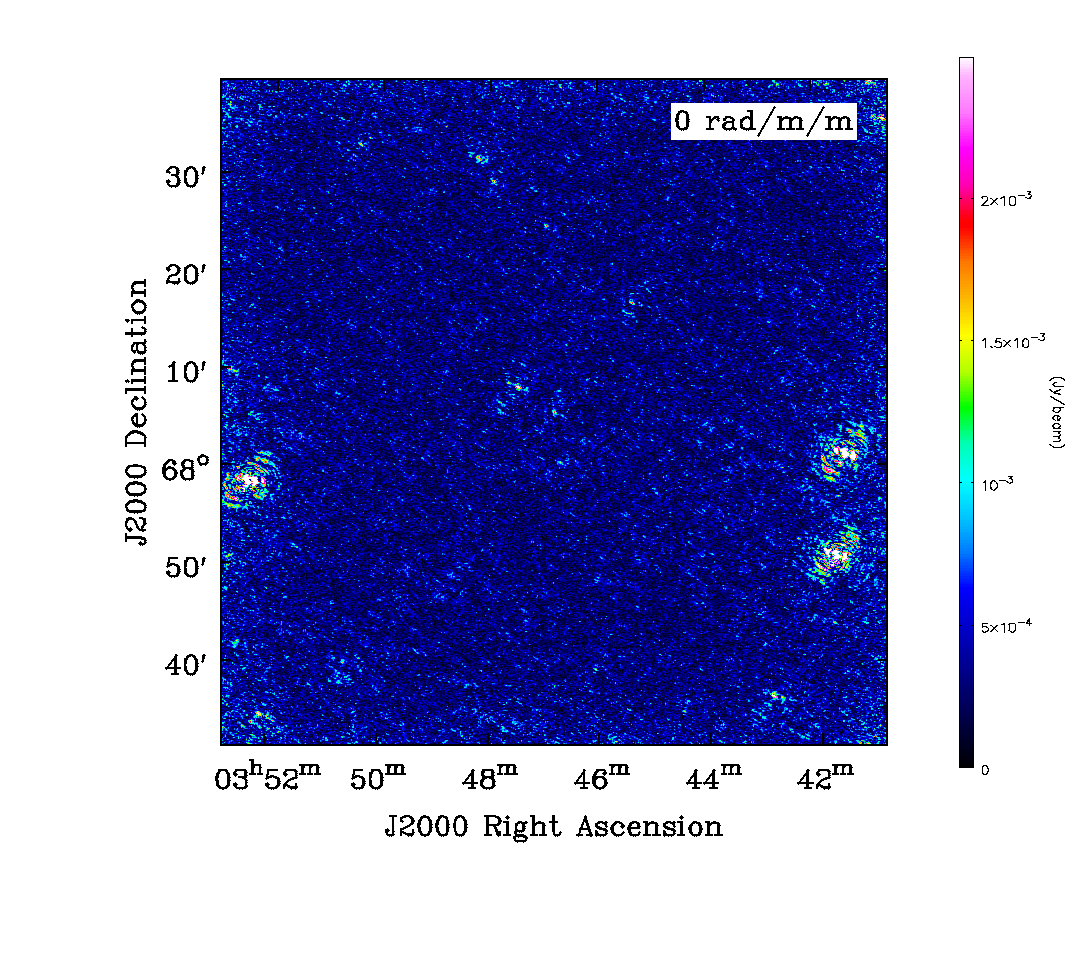
\includegraphics[scale = 0.4]{400_instr.png}
\caption{Instrumental polarization seen at the Faraday depth of 0 rad/m$^2$.}
\label{fd0}
\end{figure}

For NGC\,628 also, RM Synthesis is performed. It uses the same procedure as explained above. The resolution for the Faraday Depth is 0.814~rad/m$^2$. The maximum frequency used for this is 171.06~MHz and the minimum frequency is 110.7~MHz. The largest detectable structure is 0.695~rad/m$^2$. The cutoff is set as 0.1~mJy and 100 iterations of clean are performed. The galactic latitude of this galaxy is -45~deg. Even though this seems to be an optimistic latitude to observe polarization (compared to IC\,342 whose latitude is 10.58~deg), there is no polarization seen for this galaxy. The lack of observation of polarization from the two galaxies can be attributed to the maximum detectable structure. Any structure with a Faraday Depth larger than the values given by the equation \ref{eq2} would be depolarized.\\

Though diffuse emission has been studied using LOFAR, it is usually seen in the local interstellar medium, such as in the paper \citet{ic342_5}, in which the field of view was towards IC\,342. There is another study in the Fan region\footnote{The Fan
Region is centered near the Galactic plane at the latitude of +5~deg and longitude of 130~deg. It is a region that extends over 60 $\times$ 30~deg, and is characterized by the electric field vectors that appear to fan out from the Galactic plane near 130~deg at frequencies of 600~MHz.} in which diffuse polarized emission was observed \citep{2013A&A...558A..72I}. It is to be understood that observations of diffuse emission from the galaxy itself is very difficult because of the depolarization effects along the line of sight, and wavelength dependent depolarization. Attempts to study the diffuse emission has been done using LOFAR for M51 in \citet{2014A&A...568A..74M}, which gave a similar result as the one indicated for the aforementioned galaxies. Thus, polarization for star forming galaxies is harder to detect, and the search for detection of polarization should be concentrated on galaxies that have a higher magnetic fields with little star formation.

\subsection{Extra-galactic polarized sources}
Studying extra-galactic polarized sources would be very useful to understand the evolution of populations of radio source, which in turn would probe the evolution of magnetic fields. Comparison of the source counts in the low frequency with that of higher frequencies, would help us understand the evolution of depolarization in radio sources, and thus the evolution of magnetic fields. Source detection might also help us in discovering new pulsars in our galaxy, as they are highly polarized point sources with a very steep spectrum, as done in \citet{2015A&A...583A.137J}, in which the source J081558+461155 is discovered as a pulsar in the field of 3C 196. Pulsars appear as Faraday thin sources, as the pulsar B1112+50 that was found in the paper \citet{2018arXiv180104467V} in the LOFAR Two-meter Sky Survey (LOTSS). 
In the paper \citet{2018arXiv180104467V}, around 92 polarized sources are found in an area of 570 square degrees, i.e., 1 source per 6.2~deg. In \citet{2014A&A...568A..74M}, 6 polarized sources were found in an area of 17.3 square degrees, i.e., 1 source per 2.9 square degrees. In the paper \citet{ic342_5}, 3 polarized sources (henceforth referred to as Van Eck sources) are detected in an area of 5 square degrees, in the field of IC\,342, at the frequency of LOFAR.
\paragraph{Procedure:} In order to study the polarization of extra-galactic sources at 150~MHz, I try to make smaller Faraday cubes around the sources that have been detected in \citet{2009ApJ...702.1230T}, henceforth referred to as ``Taylor catalog". This is done because it is easier to study already detected sources, and understand their polarization and depolarization properties. This is done by first phase shifting the visibility data using the `phaseshifter' function in NDPPP. Then, with the help of \verb|pyrmsynth|, RM Cubes of these sources were made. Furthermore, I tried to manually identify sources, i.e., sources with a flux density of around 3 times the noise level of the image. One could also use the function \verb|pyBDSF|\footnote{(The Python Blob Detector and Source Finder, formerly PyBDSM) \url{http://www.astron.nl/citt/pybdsf/}} provided in casa to do the same. This is done for both IC\,342 and NGC\,628.\\
Unfortunately, I could not detect any polarization that I could be certain was true. For IC\,342, there are three sources from the Taylor catalog that were in my field of view. It is to be noted that the Van Eck sources found are all out of the field of view I am studying, and were not detected. Hence, it is of no surprise that I could not detect any polarization from the three sources present in my field of view. The table \ref{vaneck} shows the Van Eck sources. The amount of depolarization in the Van Eck sources have been calulated by me using the formula in \citet{2007A&A...470..539B}:
\begin{equation}
\textrm{DP(150,1400)} = \frac{\textrm{PI}_{150}/\textrm{PI}_{1400}}{(\nu_{1400}/\nu_{151})^{\alpha}}
\label{DP}
\end{equation}
Here, PI$_{1400}$ is the polarization intensity at 1.4~GHz as given in the Taylor catalog, and PI$_{150}$ is the polarized intensity of the Van Eck sources. A value of 1 represents no additional depolarization has been seen at 150~MHz, while a value of 0 represents that the source is completely depolarized.
\begin{table}
        \centering
        \begin{tabular}{cccccccc}
        \hline\hline
            RA$^a$ & DEC$^b$ & PI$_{150}^c$ & PI$_{1.4}^d$ & RM$_{150}^c$ & RM$_{1.4}^d$ & I$_{1.4}^d$ & DP\\
            03 17 47.08$\pm$ 0.11 &  +68 25 08.30$\pm$7 &33.45$\pm$0.89 & 15.4$\pm$0.7 & -11.4$\pm$0.05 & -32.9$\pm$15.8 & 168.4$\pm$5.7 & 0.131
\\
			03 17 42.46$\pm$0.08 &  +68 24 33.30$\pm$6 &32.93$\pm$1.04 & 14.6$\pm$0.7 & -8.6$\pm$0.05 & -12.8$\pm$4.7 & 222.3$\pm$7.2 & 0.060
\\
			04 14 45.39$\pm$0.09 &  +69 01 08.30$\pm$6 &5.67$\pm$0.37 & 8.0$\pm$0.5 & -28.6$\pm$0.05 & -32.9$\pm$15.8 & 115.7$\pm$4.1& 0.124
\\
            \hline
        \end{tabular}
        \caption{$a$ and $b$ represent the RA and DEC as given the the Taylor catalog. $d$ is from the Taylor catalog, while $c$ is the quantity of the Van Eck source. The degrees of depolarization is given in the last column using the equation \ref{DP}.}
        \label{vaneck}
    \end{table}

\noindent The values of degree of depolarization are similar to the ones in the paper \citet{2014A&A...568A..74M}, in the field of M51\footnote{0.038, 0.196 and 0.029 (not for the aforementioned sources!)}. One cannot make a conclusion as to why some of the sources in the Taylor catalog cannot be seen the this frequency, as some of the sources that are present in my field of view have a polarized intensity from around 25 to 8~mJy, with a flux density of almost 600~mJy to 42~mJy (see table \ref{tay}), that are in the range of the quantities of Van Eck sources. In the paper \citet{2014A&A...568A..74M}, polarization from sources with polarized intensity as low as 0.89~mJy has been studied, with the integrated flux density of one of the sources as low as 44~mJy.\\

\begin{table}
        \centering
        \begin{tabular}{cccccccc}
        \hline\hline
        RA$^a$ & DEC$^b$ & I$_{1.4}^d$ & PI$_{1.4}^d$ & RM$_{1.4}^d$ \\
03 52 23.34$\pm$0.08 & +67 58 27.80$\pm$0.6 & 587.5$\pm$18.7 & 25.17$\pm$0.31 & -11.2$\pm$2.5\\
03 52 14.00$\pm$0.1	& +67 58 39.80$\pm$0.6	& 42.4$\pm$1.3 & 8.02$\pm$0.37 & -13.8$\pm$7.9\\
03 41 30.77$\pm$0.08 & +68 01 21.40$\pm$0.6	& 342.6$\pm$12 & 11.88$\pm$0.3 & -32.2$\pm$5.3\\
\hline
        \end{tabular}
\caption{All these sources are from the Taylor catalog, which are present in my field of view. They are not polarized at 150~MHz in my study.}
        \label{tay}
    \end{table}
For NGC\,628, there are 34 sources from the Taylor catalog that are in the field of view. Similar procedure as the one for IC\,342 is followed. None of these sources are seen to have any polarized emission. The Faraday spectrum of one of the sources is given in the Figure \ref{FS}. This is most probably an an AGN source, as can be seen in the Figure \ref{source11}. It has a peak polarized intensity of 7.32~mJy and a flux density of 112.7~mJy. It is one of the hihger values among the other sources present in the field of view, and is expected to show polarization at 150~MHz frequency range. However, no clear peak can be seen in the Faraday spectrum. \\

\begin{figure}[h]
\centering
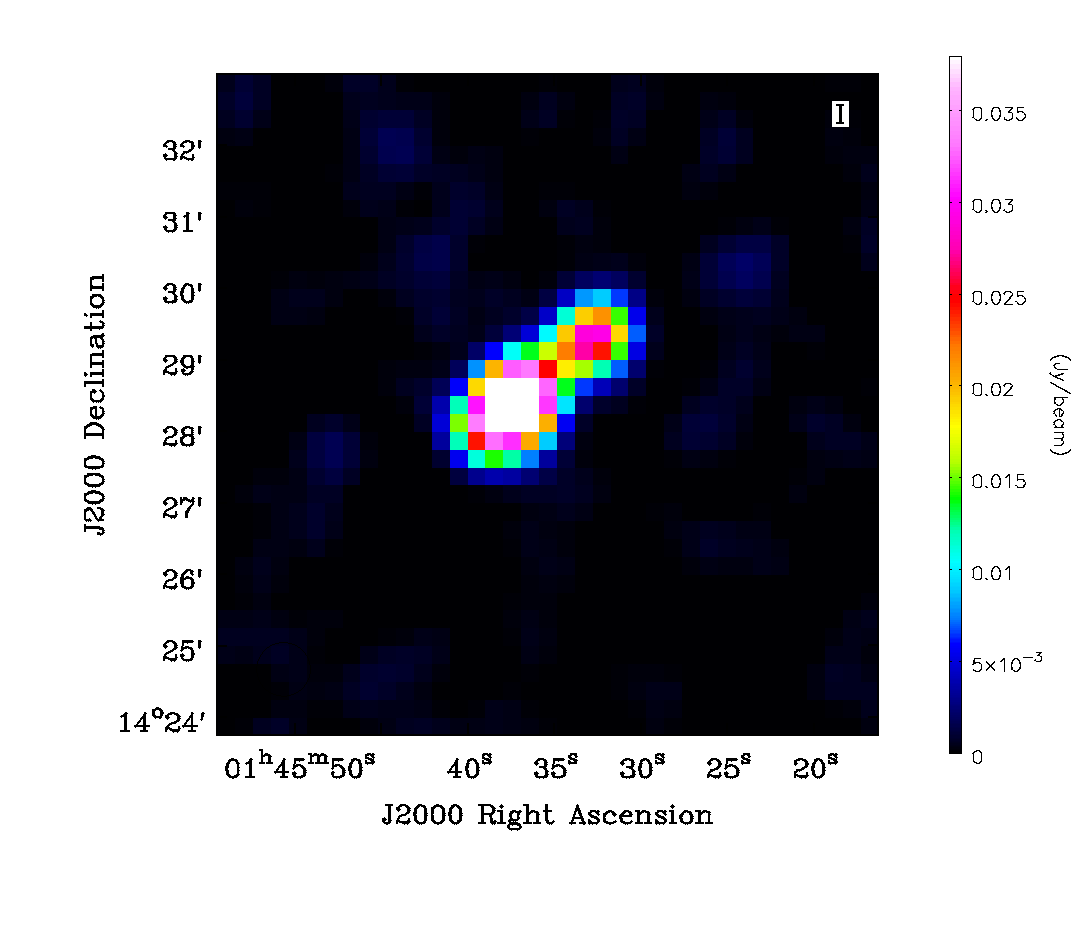
\includegraphics[scale = 0.4]{source11.png}
\caption{One of the sources from the Taylor catalog that has been observed to have a higher polarized intensity compared to other sources in the FoV of NGC\,628 (7.32~mJy). It is expected to be polarized at 150~MHz, but no polarization is seen. This image has been taken from the NVSS survey and is at a frequency of 1.4~GHz.}
\label{source11}
\end{figure}

\begin{figure}[h]
\centering
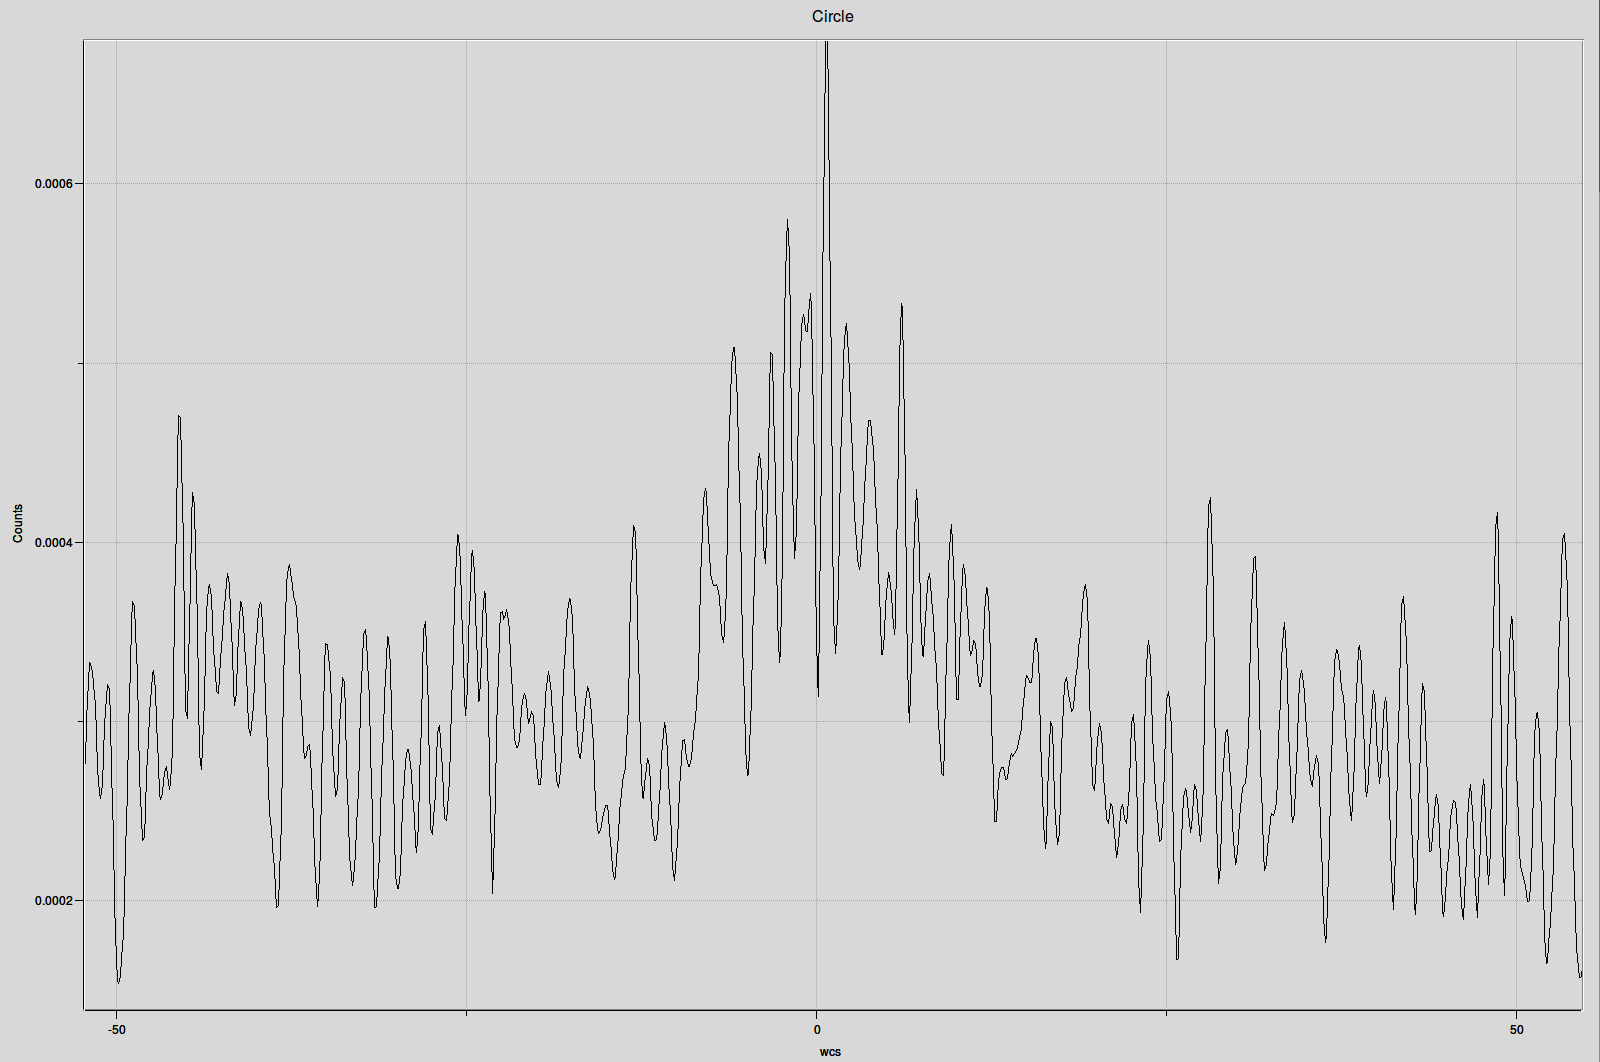
\includegraphics[scale = 0.2]{-50to50.png}
\caption{Most of the Faraday Spectrum that has been studied looks like this, thus making it impossible to understand if there are any real peaks in the Faraday spectrum.}
\label{FS}
\end{figure}
\noindent In order to identify, I use the code provided by Dr. S.P O' Sullivan (priv. communication), which uses the method described in \citet{2012PASA...29..214G} to detect sources. I first try to set the detection threshold for the smaller RM Cubes as 8$\sigma_{QU}$. This provides no results. Similar results are obtained for the thresholds of 7$\sigma_{QU}$, 5$\sigma_{QU}$, 3$\sigma_{QU}$ and finally 2$\sigma_{QU}$. The $\sigma_{QU}$ value is calculated by the code, which uses the noise value from the Faraday depths over beyond +100 and less than -100, as no polarized sources has been detected at such high and low Faraday depths. The Faraday depths from -5 to +5 are avoided due to the presence of instrumental polarization effects. I try the same for most of the sources in the field of view that are present in Taylor catalog, with negative results. 
\end{document}
